\chapter{Technology} 

Many technologies were examined and experimented with and the positives and
negatives of each was weighed up before a decision about
suitable choice for the visualisation was made. It came down to 3 potential
technologies
that
would be suitable, the next 3 subsections outline these in
detail.

\section{Processing - Chosen Technology}
Processing is an open source programming language and development environment
that was created to teach the fundamentals of computer programming with a visual
context.
Using processing would mean that the visualization could be built with Java
while still using
an effective visualisation framework that supports 3D elements. The most
complete existing visualization
using
the same exoplanet dataset (The Kepler Visualization Tool) is built using
Processing.
Using this solution would involve learning the semantics of Processing but as it
is a library built in Java so the syntax is the same with only minor changes.
This means the learning
curve should be shallow.

\section{D3 (Data Driven Documents) - Alternate Technology}
D3 is a JavaScript library that allows the data to be displayed in dynamic
graphics. Embedded
within an HTML web page, the JavaScript D3.js library uses pre-built
functions to
select elements, create Scalable Vector Graphics (SVG) [17] objects, style them,
and add transitions,
dynamic effects, and tooltips. Large datasets can be easily bound to SVG objects
using
simple D3 functions to generate rich charts and diagrams. D3 was created because
of the
need for a balance of expressiveness, efficiency, and accessibility that
previous visualization
toolkits did not allow [4].

D3 allows the binding of input data to arbitrary input elements. This means that
the exoplanet dataset can easily be bound to SVG elements to create a
visualisation. D3
adopts the W3C Selectors API to identify document elements queried. This results
in a
rich but concise selection method of elements in a visualisation. It allows
debugging thanks to Google chrome and other modern browsers
development tools. A downside to D3 is that it does not allow 3D diagrams,
although it does
allow pseudo 3D by using the painters algorithm and 3D textures.

\section{Prefuse - Alternate Technology}
Prefuse is a set of software tools for creating rich interactive data
visualizations [13]. The
Prefuse toolkit provides a visualisation framework for Java. It supports a set
of features
for visualising and interacting with data. It can be used to build standalone
applications, visual
components embedded
in larger applications, and web applets. Prefuse to greatly simplifies the
process
of representing and efficiently handling data, mapping data to visual
representations (e.g.,
through spatial position, size, shape, color, etc), and interacting with the
data.
To use Prefuse a basic familiarity with the Java is required, including setting
up and building
Java projects. A knowledge of Swing or another similar user interface toolkit is
also
useful for understanding some of the concepts behind Prefuse and for integrating
Prefuse
visualisations into larger applications. Prefuse is a very powerful tool that
has a very high learning curve due
to the amount of development power that it has. This means that learning it and
using it pushes it out of scope for this project.


\section{Decision of technology}

The technology chosen needed to offer a combination of low learning curve,
strong visualisation ability, and 3D support.
The final technology decision was to use Processing, this is because it had all
of the desirable qualities that this project required as Figure \ref{fig:
techChoices} shows. 

\begin{figure}[H]
  \centering
      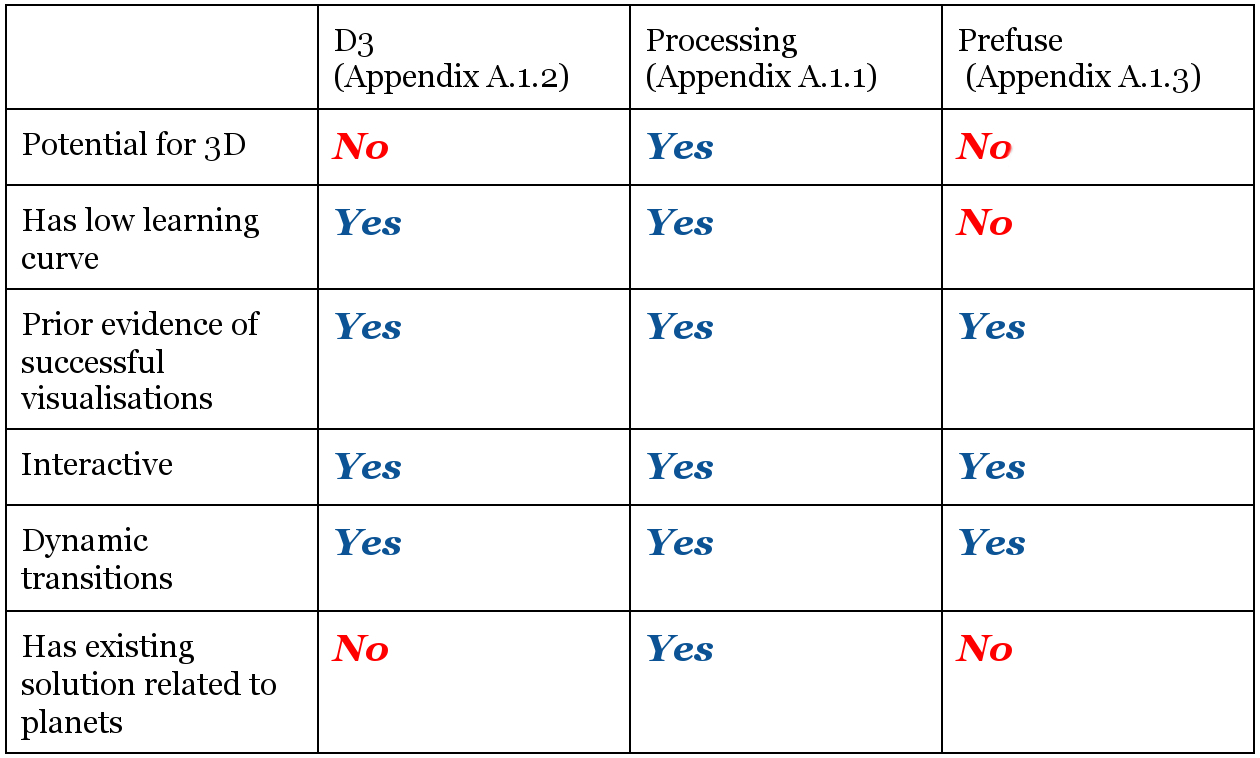
\includegraphics[width=0.8\textwidth]{images/table_technologies.jpg}
  \caption{Table of technology choices}
  \label{fig: techChoices}
\end{figure}

By choosing Processing, it allowed me to extend a an existing visualisation
using the same data set, The Kepler Visualisation Tool in Section \ref{sec:kep}.
Building upon an existing solution allowed the project to progress faster
towards fulfilling the project requirements as less of the groundwork needed to
be carried out. This was a large advantage as doing this groundwork would limit
the amount time that could be spent on new features.


